% Author: Till Tantau
% Source: The PGF/TikZ manual
\documentclass[a4paper,11pt]{article}
\usepackage[utf8]{inputenc}
\usepackage{listings}
\usepackage{amsmath}    % need for subequations
\usepackage{graphicx}   % need for figures
\usepackage{verbatim}   % useful for program listings
\usepackage{color}      % use if color is used in text
%\usepackage{subfigure}  % use for side-by-side figures
\usepackage{hyperref}   % use for hypertext links, including those to external documents and URLs
\usepackage{url}
\usepackage{float}
\usepackage{todonotes}
\usepackage{tikz}
\usepackage{enumitem}
\usepackage{hyperref}
\usepackage{pdfpages}
\usepackage{caption}
\usepackage{epsfig}
\usepackage{subcaption}
\usepackage{listings}
\usepackage{color}
\usepackage{amsfonts}
\usepackage{latexsym}
\usepackage[T1]{fontenc} % use for allowing < and > in cleartext
\usepackage{fixltx2e}    % use for textsubscript
\usepackage[linesnumbered,boxed,ruled]{algorithm2e}
\usepackage{mathtools}
\DeclarePairedDelimiter{\ceil}{\lceil}{\rceil}
%\newcommand{\BigO}[1]{\ensuremath{\operatorname{O}\left(#1\right)}}
\newcommand{\BigO}[1]{\ensuremath{\mathop{}\mathopen{}\mathcal{O}\mathopen{}\left(#1\right)}}

\definecolor{mygreen}{rgb}{0,0.6,0}
\definecolor{mygray}{rgb}{0.5,0.5,0.5}
\definecolor{mymauve}{rgb}{0.58,0,0.82}
\lstset{ %
  backgroundcolor=\color{white},   % choose the background color; you must add \usepackage{color} or \usepackage{xcolor}
  basicstyle=\footnotesize,        % the size of the fonts that are used for the code
  breakatwhitespace=false,         % sets if automatic breaks should only happen at whitespace
  breaklines=true,                 % sets automatic line breaking
  captionpos=b,                    % sets the caption-position to bottom
  commentstyle=\color{mygreen},    % comment style
  deletekeywords={...},            % if you want to delete keywords from the given language
  escapeinside={\%*}{*)},          % if you want to add LaTeX within your code
  extendedchars=true,              % lets you use non-ASCII characters; for 8-bits encodings only, does not work with UTF-8
  %frame=single,                    % adds a frame around the code
  keepspaces=true,                 % keeps spaces in text, useful for keeping indentation of code (possibly needs columns=flexible)
  keywordstyle=\color{blue},       % keyword style
  language=Octave,                 % the language of the code
  morekeywords={*,...},            % if you want to add more keywords to the set
  numbers=left,                    % where to put the line-numbers; possible values are (none, left, right)
  numbersep=5pt,                   % how far the line-numbers are from the code
  numberstyle=\tiny\color{mygray}, % the style that is used for the line-numbers
  rulecolor=\color{black},         % if not set, the frame-color may be changed on line-breaks within not-black text (e.g. comments (green here))
  showspaces=false,                % show spaces everywhere adding particular underscores; it overrides 'showstringspaces'
  showstringspaces=false,          % underline spaces within strings only
  showtabs=false,                  % show tabs within strings adding particular underscores
  stepnumber=2,                    % the step between two line-numbers. If it's 1, each line will be numbered
  stringstyle=\color{mymauve},     % string literal style
  tabsize=2,                       % sets default tabsize to 2 spaces
  %title=\lstname                   % show the filename of files included with \lstinputlisting; also try caption instead of title
}

\bibliographystyle{plain}
\begin{document}
\graphicspath{ {./images/} }
\date{May 21st 2014}
\title{Extending Distance Sensitive Bloom Filters}

\author{Marcus Gregersen\\
\texttt{mabg@itu.dk}
\and Martin Faartoft\\
\texttt{mlfa@itu.dk}
\and Rick Marker\\
\texttt{rdam@itu.dk}\thanks{Supervisor: Rasmus Pagh \texttt{pagh@itu.dk}}}
%TODO vejleder og institut
\clearpage\maketitle
\thispagestyle{empty}
\setcounter{page}{1}
\begin{abstract}
We consider the Similarity Search problem, in which we, given some universe of elements $S$ and a query element $q$, would like some data structure to answer 'close' if some element in $S$ matched $q$ on at least an $\epsilon$-fration of the attributes of $q$.

This problem can be solved using Distance-Sensitive Bloom Filters as described by Kirsch and Mitzenmacher\cite{paper:harvard}.

We contribute three extensions to the DSBF data structure. We improve the robustness by modifying the Locality Sensitive Hashing functions, so they sample bits in a systematic and balanced way.

We provide a guarantee against false negatives, if bit sampling is balanced and the threshold $t$ is chosen correctly. We show that this is a tradeoff resulting in an increased probability of false positives, and is conclude that this is only useful for very small values of $\epsilon$.


Finally we extend the DSBF structure to also support queries with wildcards. We show that this can be done with no additional space, and a slight increase the false positive rate. Wildcard search makes the running time of a query exponential in the number of wildcards, but we show that if the number of wildcarded bits is chosen correctly, the expected running time becomes constant.
\end{abstract}

%\newpage
%\setcounter{page}{1}

\section{Introduction}
In the following we investigate the Similarity Search problem. Different approaches have been explored by earlier work, and in this paper we consider two of those; 'Distance-Sensitive Bloom Filters'\cite{paper:harvard} by Kirsch and Mitzenmacher, and 'Locality-Sensitive Bloom Filter for Approximate Membership Query'\cite{paper:hua} by Hua et al.

\subsection{Problem Definition}
The Similarity Search problem can be stated as follows: Given a set of elements $S$, determine if there exists an element $s \in S$ that is 'close' to a given query element $q$. Where 'close' is defined as being within a given distance, $d$ using a certain metric.

A real-word example could be a database of candidates used by a headhunting agency. Each candidate in the database would then have a set of attributes, for example \{\texttt{age}, \texttt{gender}, \texttt{race}, \texttt{education}, and \texttt{experience}\}.
An application of Similarity Search can then be formulated as: "Given some person P, does the database contain one or more candidates, similar to P?".
% Begræns problemet
In the following we consider the Similarity Search problem for bit-vectors of length $l$, and Hamming distance as metric. This reduction maintains a high degree of generality, since elements from any domain can be encoded as bit-vectors.

\subsection{Key Concepts}
\label{sec:lsh}
\begin{description}
\item[Hamming distance]

A distance metric for bit-vectors. The Hamming distance between two vectors $v_1, v_2$ is given as the number of positions $i$ where $v_1[i] \neq v_2[i]$

\item[Bloom filters]
A compact, but inexact set representation. It answers membership queries in constant time, but allows for false positives, meaning it can either answer "Maybe in the set", or "Definitely not in the set".\footnote{See \cite{paper:bloom} for details on Bloom filters}

\item[Locality Sensitive Hashing]
Ordinary hashing tries to minimize the probability of a collision, while Locality-Sensitive Hashing (LSH) attempts to maximize the collision probability for sufficiently similar elements.

LSH functions are not known for all similarity-measures, but for the Hamming metric on bit-vectors, a particularly simple one is known: Sample a fixed number of bit positions, $l'$, from the input bit-vector, uniformly at random.
This LSH now considers all vectors that are identical on the $l'$ sampled bit positions, identical. This type of collision is highly desired (called locality collision in the following). Storing all of these requires $2^{l'}$ space, which is not feasible for large values of $l'$. The solution is to hash the bit vector to an integer, and use that value as an index in some array of size $m$. When $m < 2^{l'}$, we have from the pigeonhole principle, that multiple bit vectors must hash to the same value, similar to ordinary hashing collisions. This type of collision is not desirable, and leads to an increase in false positives. We call this an accidental collision in the following.
\end{description}

\section{Related work}

\subsection{Distance-Sensitive Bloom Filters}
Kirsch and Mitzenmacher propose in the paper 'Distance-Sensitive Bloom Filters'\cite{paper:harvard} a novel way of using Bloom filters. The aim is to expand upon classical Bloom filters, enabling them to solve the Similarity Search problem. They note that such a data structure has a number of practical uses, if it can be made sufficiently effective in both time and space.

Like Bloom filters, the DSBF structure supports two operations:
\texttt{Insert} which adds an element to the set, and \texttt{Query} which queries the DSBF for the existence of similar elements.
The \texttt{Query} operation should return:
\begin{itemize}
\item 'close' if an element in the set differs from the query element in at most an $\epsilon$-fraction of the bits.
\item 'not close' If every inserted element, differs from the query element in at least a $\delta$-fraction of the bits.
\item either 'close' or 'not close', if the fraction of differences lies between $\epsilon$ and $\delta$.
\end{itemize}

They accomplish this by using $k$ locality sensitive hashing functions, independently chosen such that two elements that are sufficiently similar, will hash to the same value with a high probability.
When querying the Bloom filter for an approximate match, the element is hashed with each of the LSH functions, and the corresponding indiceses are checked. If there are more bits, than a specified threshold ($t$), that is set to 1, it returns that the data contains an element that is close to the query element. In contrast to standard Bloom filters, the usage of LSH introduces the possibility of false negatives, due to accidental LSH collisions, but the use of a threshold keeps the false negative probability fairly low.

\begin{figure}[H]
\centering
  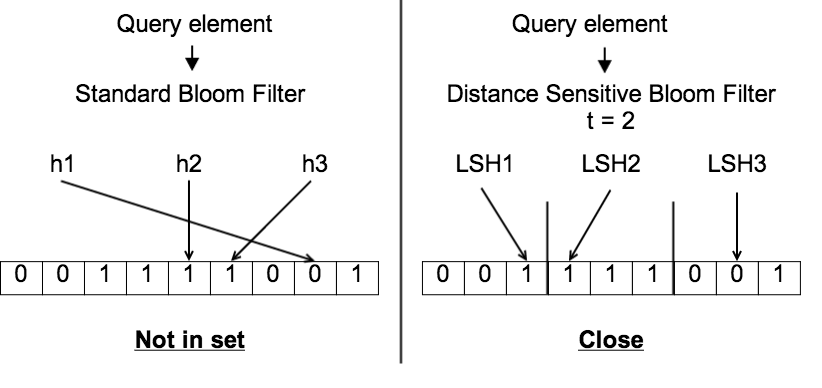
\includegraphics[width=.95\linewidth]{sbf_vs_dsbf}
\caption{Comparing Bloom filter and DSBF when querying}
\label{fig:sbf-vs-dsbf}
\end{figure}

Figure \ref{fig:sbf-vs-dsbf} shows the differences between querying a standard Bloom filter, and a DSBF.\\

In their experiments they manage to achieve false postive rates and false negative rates of 1.5\% and 0.2\% respectively for 1000 elements, with $\epsilon = 0.1$ and $\delta = 0.4$. For 10000 elements they achieve 0.016\% false positive rate and 0.003\% false negative rate, with with $\epsilon = 0.05$ and $\delta = 0.4$. For 1000 elements they use 64\% of the total space of the elements, and for 10000 elements they use 51\% of the total space.

\subsection{Locality-Sensitive Bloom Filter for Approximate Membership Query}
The paper written by Hua et al.\cite{paper:hua} introduces the 'Locality Sensitive Bloom Filter'. This builds on \cite{paper:harvard}, but takes a somewhat different approach. They use a standard Bloom filter data structure, with LSH functions in place of ordinary hash functions, but choose to not apply thresholding. This approach, has a high probability of both false positives and false negatives, since every single LSH has to agree on every answer. To minimize these, they introduce a pair of auxiliary data structures, as described in the following.

\paragraph{Minimizing False Positives}
Every time an element $q$ is checked for approximate membership, the LSBF is checked. If every bit in the array that $q$ hashes to is set to $1$, that could mean one of two things.
1) An element $p$ exists in the LSBF, that is approximately close to $q$ (a true positive)
2) Multiple elements added to the LSBF, together, have set all the bit positions corresponding to $q$ to $1$, and no single element is approximately close to $q$. (a false positive).

To minimize the probability of a false positive, a Verification Scheme (VS) data structure is added.
This is a standard Bloom filter (ordinary hashing, not LSH), and is maintained as follows: Every time an element is added to the LSBF, the bit positions that corresponds to that element, are encoded (see figure \ref{fig:verification_scheme}) and inserted into the VS Bloom filter.
When the LSBF is queried, it first verifies that all bits corresponding to the query element $q$ are set to $1$ in the LSBF, then it encodes the bit positions (Figure \ref{fig:verification_scheme}), and queries the VS for an exact match. If an exact match for the encoded version of $q$ is found in VS, then it is highly likely that a single element $p$ is responsible for setting all the bits in the LSBF, and the query will return 'close'. If, on the other hand, the VS does not contain an element that matches the encoded $q$, then multiple elements must be responsible for the bits being set, and the query will return 'not close', preventing a false positive.

\begin{figure}[H]
\centering
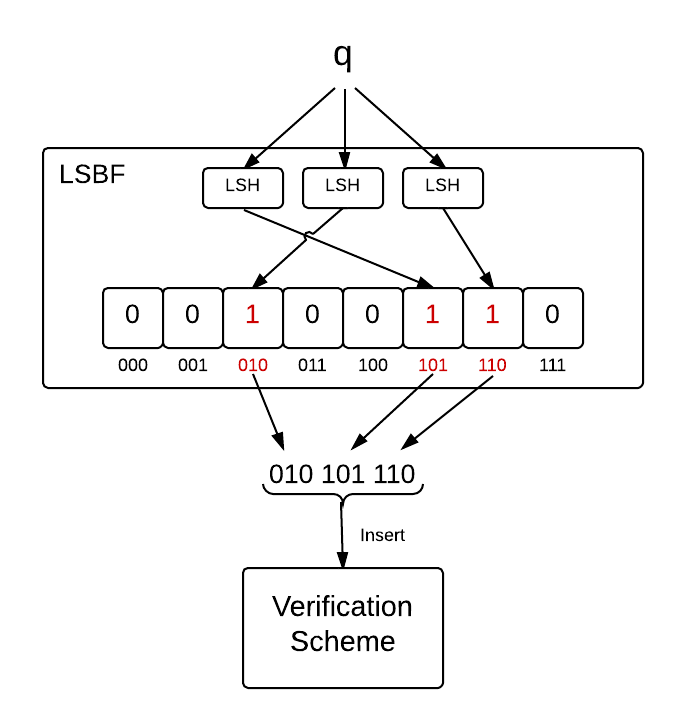
\includegraphics[width=.5\linewidth]{verification_scheme}
\caption{Maintaining the Verification Scheme, when adding elements to an LSBF}
\label{fig:verification_scheme}
\end{figure}

Note that since the Verification Scheme is a standard Bloom filter, it is susceptible to false positives itself. this means it only serves to minimize false positives, not prevent them completely.

\paragraph{Minimizing False Negatives}
Hua et al. use a method called Active Overflowed Scheme. The idea is that, while a pair of close elements may not be hashed to the same value, they may instead hash to values that are adjacent in the bit array. So when querying, instead of just looking at the bits which represents the hashed element, they also check the $t$ closest bits to either side. $t$ will depend on the price of false positives compared to false negatives as this approach will introduce more false positives\footnote{We remain sceptical towards the Active Overflowed Scheme. We see no reason for LSH values to exhibit 'neighbour' locality, unless a difference happens to be in the least significant bit.
}.\\

In their paper, Hua et al. have chosen to use a 'proximity measure', which makes it difficult to compare the results to the ones found in \cite{paper:harvard}. Furthermore, all results are only presented in graph form. From the graphs, however, we can see that they achieve between 85\% and 100\% accuracy.\\


In the following, we will build upon the work of \cite{paper:harvard}.  Their work achieves robustness by using thresholds and the way they present their results allows for easy comparison.\\

We will not be discussing the paper of Hua et al.\cite{paper:hua} further. They provide no clear description on how they construct their LSH's, and they provide only plotted data, making comparisons difficult. Furthermore, it is unclear to us how they are able to implement the Active Overflowed Scheme.

\section{Naïve Solutions for Similarity Search} \label{naive_approaches}

\subsection{Linear Scan}
The most obvious idea for solving the Similarity Search problem, is to apply brute force.
Let $n$ be the number of elements in $S$, $n = |S|$.
The idea is to store the elements $S$ in a linked list. When a query is made, scan the linked list, and calculate the distance from each element $s \in S$ the query element $q$. If $s$ satisfies the distance requirement, a match has been found. If the end of the linked list is reached, no match exists.
This yields a time and space complexity of \BigO{n}.\\

This will give a correct answer, and will work well for small problem instances, But the linear requirement on time and space is prohibitively expensive for many real-world applications.

\subsection{Bloom filters} If we relax the requirements on space or time, we can change these characteristics to support either constant-time queries, or space-efficiency, but not both.\\

While keeping in mind that standard Bloom filters only supports exact matches, we see that one way of achieving this is by relying on extra insertions. Every time an element is inserted into the Bloom filter, all elements within distance $d$ are generated and added in addition to the original element. This increases the space requirement for the DSBF, and the time complexity of the \texttt{Insert} operation to be \BigO{2^d}, while keeping the time complexity of \texttt{Query} at \BigO{1}.\\

Another tradeoff is to sacrifice time when querying. This can be done by generating all elements within distance $d$ of the element we are comparing to, and run a query for each. This approach has the benefit of being space efficient, and offering constant time for \texttt{Insert}, but will cause the time complexity of \texttt{Query} to increase to \BigO{2^d}.\\

%specifikt for naive bloom filtre
The exponential time / space complexities makes this unusable for non-trivial problem sizes.

\section{Balanced LSH Bit Sampling} \label{sec:balanced}

The default way to initialize the LSH functions used in the Distance-Sensitive Bloom filter (DSBF), is for each of the $k$ LSH functions, to choose $l'$ bit positions to sample, uniformly at random. On average this should spread the sampled bits out nicely across the $k$ hash-functions, but in some cases this will result in a skewed distribution, meaning that some bits are oversampled, while others may not be sampled at all. We believe that this will degrade the performance of the DSBF, resulting in more false positives and -negatives.

Inspired by ideas from our supervisor we investigate how this may be improved upon.

By initializing the LSHs such that all bit positions are sampled equally often, we can avoid the problems arising from unbalanced bit sampling.
In practice we do this by first preparing a vector of length $k \cdot l'$ by repeating the the integers from 0 to $l$ as many times as required. We then shuffle the vector, and assign each of the $k$ functions a sub-vector of length $l'$, making sure that every index in the sub-vector is unique. This preprocessing step takes $O(l)$ time, and protects the DSBF from poor performance due to skewed sampling.

\subsection{Experiments}
Figure \ref{fig:bitbalance-fpnr} shows an experiment run with Balanced bit sampling enabled (illustrated by the solid black line) and disabled (illustrated by the dashed red line), and shows that this optimization in some cases improves the performance of the DSBF.

In practice, when $l$ get sufficiently large, the probability that a DSBF without bit balancing will produce a skewed sampling becomes infinitesimal.
\begin{figure}[H]
\centering
\begin{subfigure}{.5\textwidth}
  \centering
  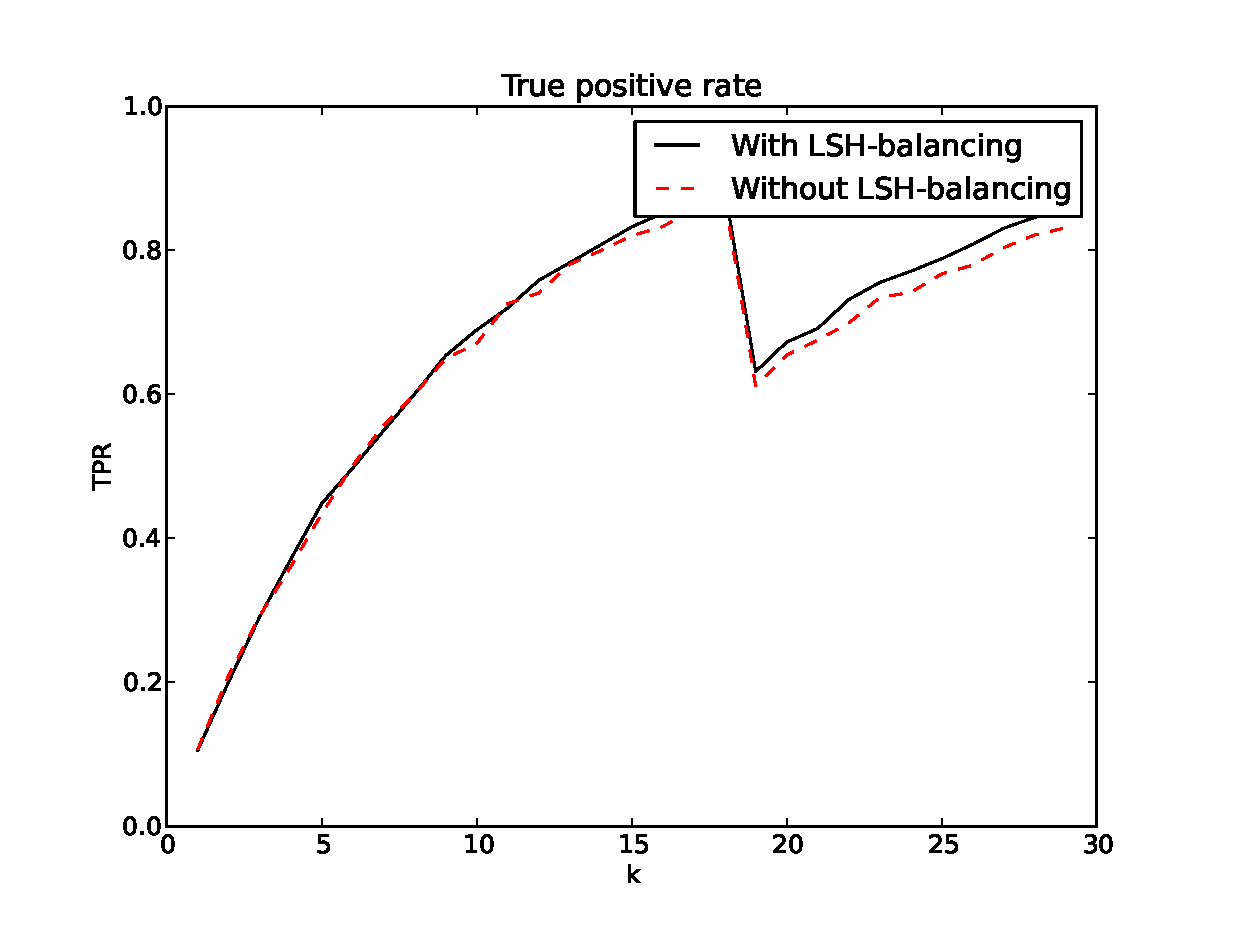
\includegraphics[width=.95\linewidth]{bitbalancing_TPR1}
\end{subfigure}%
\begin{subfigure}{.5\textwidth}
  \centering
  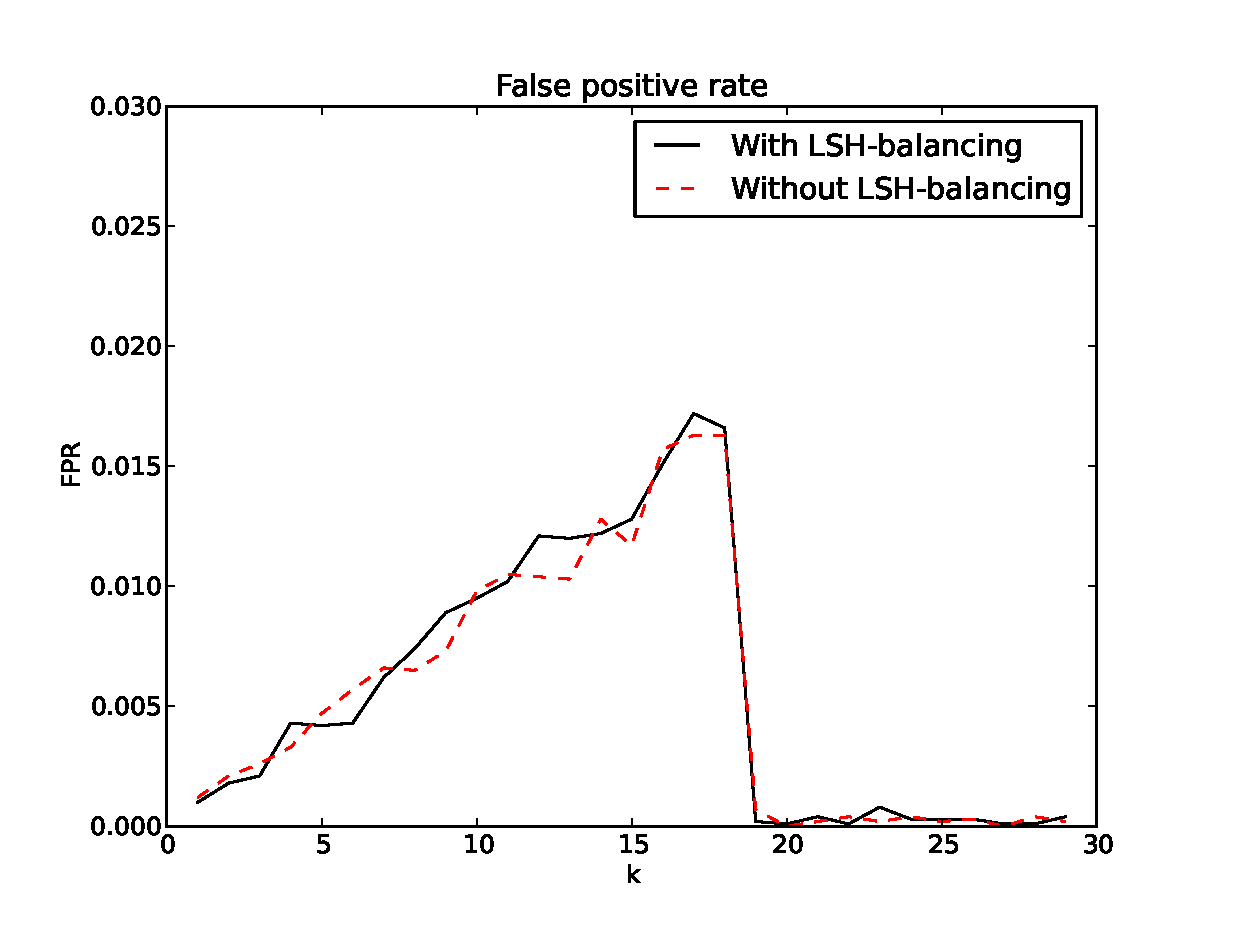
\includegraphics[width=.95\linewidth]{bitbalancing_FPR1}
\end{subfigure}
\begin{subfigure}{.5\textwidth}
  \centering
  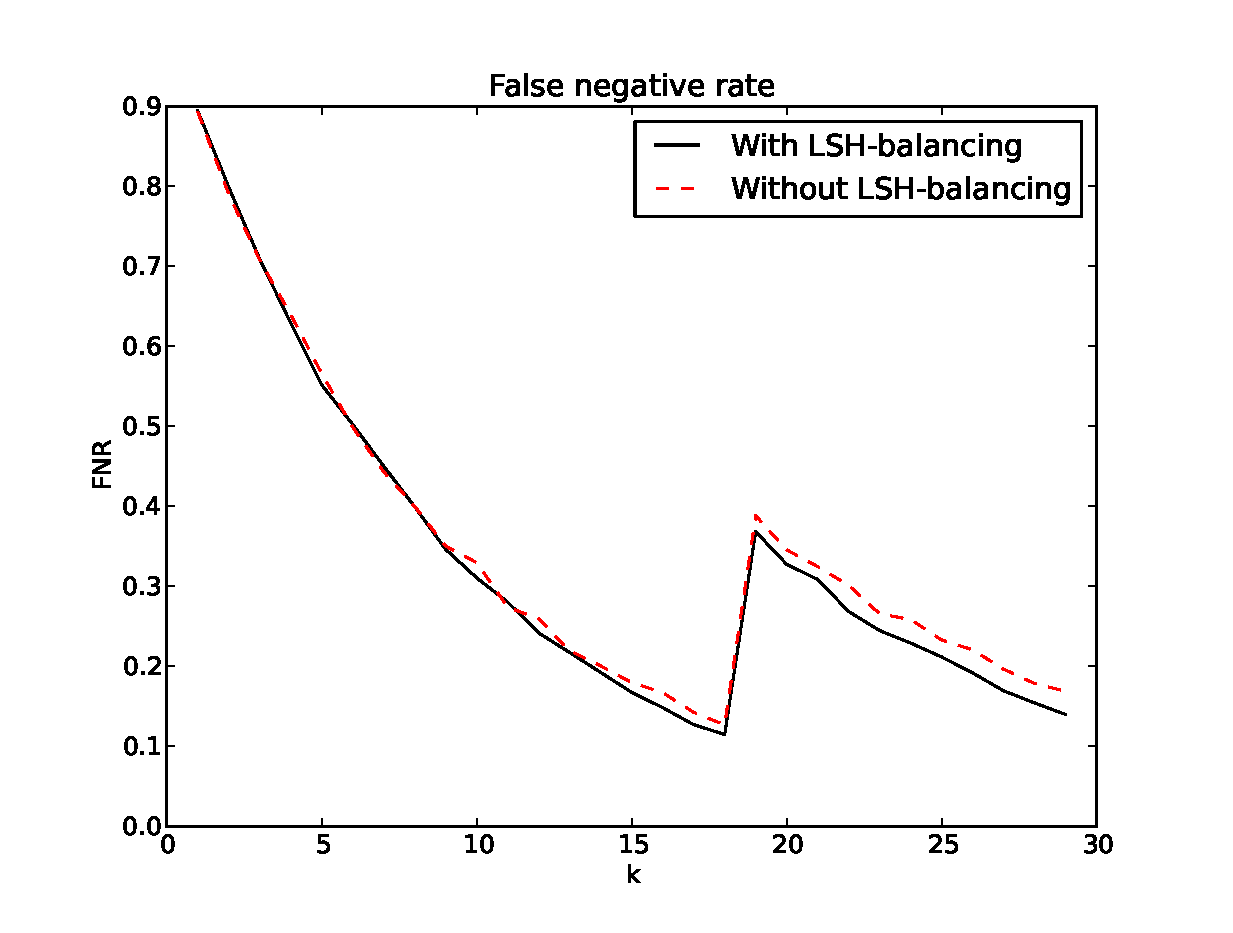
\includegraphics[width=.95\linewidth]{bitbalancing_FNR1}
\end{subfigure}
\caption{The observed true positive, false positive and false negative rates for $n$ = 1000, $l$ = 1000, $\epsilon$ = 0.1, and $\delta$ = 0.4, with LSH bit-balancing enabled and disabled}
\label{fig:bitbalance-fpnr}
\end{figure}


\section{Eliminating False Negatives}
Building on the previous idea from Section \ref{sec:balanced}, we present a method to eliminate false negatives from the DSBF data-structure.

False Negatives \label{p:fn}happen when a query element is within distance $\epsilon$ of an element in S, but is reported as being 'not close'. This happens when too many of the $k$ LSH functions report false, driving the number of trues below the threshold $t$. We know that each of the LSHs that report false, will sample at least one bit in which $q$ and every element $s \in S$ differ. Since q, by definition, is 'close' to some element $s \in S$, the maximum number of differences between $q$ and the closest element in $S$ is: $\epsilon_{abs} = \ceil{\epsilon \cdot l}$, where $l$ is the element length. Assuming that each is sampled an equal number of times (ensured by \ref{sec:balanced})): $n_{sample} = \ceil{\frac{k \cdot l{'}}{l}}$, the maximum number of hash-functions that can report false is: $n_{false} = e_{abs} \cdot n_{sample}$.

Providing a guarantee against false negatives can be achieved by lowering the DSBF threshold appropriately. Given the knowledge of $n_{false}$, we can set $t = k - n_{false}$, and thereby eliminate the possibility of false negatives completely.

Lowering $t$ comes at a price. The lower the value of $t$, the higher the probability of a false positive. In the edge case, where $t=0$, the DSBF becomes useless, answering 'close' to every query. Taking this into account, we have to constrain the value of $n_{false}$ such that $t>0$.
\[t > 0 \Leftrightarrow k > n_{false} \Leftrightarrow k > \epsilon_{abs} \cdot n_{sample}\]
Since $k$ is usually chosen around $20$, and $n_{sample}$ is small and grows proportionally to $k$, $e_{abs}$ will have to be very small (below 10) for $t$ to remain positive. This limitation seriously hinders the real-world applications of the guarantee against false negatives.

\section{Wildcard Search}
The DSBF structure can, as we have seen, be used to answer questions of the form "does $S$ contain an element that is 'close' to $q$". A natural extension to this, is be able to ignore certain bits in $q$, when calculating the similarity.

If we examine the job applicants example from the introduction, an application of Similarity Search with wildcards can be formulated as follows: Given a person with attributes \{\texttt{age}, \texttt{gender}, \texttt{race}, \texttt{education}, \texttt{experience}\} does the dataset contain one or more similar applicants, disregarding the attributes \texttt{gender} and \texttt{age}.\\

The extended problem can be formally stated as: Let $W$ be a set of wildcard bit positions:
\[\forall w \in W (w \in \mathbb{Z}^+ \land w < l)\]
Given a set of elements $S$, a query element $q$ and a set of wildcards $W$. Determine if there exists an element $s \in S$ that is 'close' to $q$, not counting differences on wildcard positions $W$. Where 'close' is defined as being within a given distance, $d$ using a given metric.

\subsection{Solving Wildcard Search}
We have identified two approaches to solving the extended problem.
\subsubsection*{LSH filtering}
 The first approach is to ignore the output from all LSH's that sample one or more wildcard bits. This can be done without modifying the insertion of elements into the DSBF, and without storing additional data. However, it raises some troublesome questions.

\begin{itemize}
\item How should the threshold be chosen, when the number of ignored LSH's changes from query to query?
\item How should the bits to sample for each LSH be chosen, to minimize the probability that the LSH's that are ignored due to wildcarding, are not the only ones sampling some bit position $p \notin W$?, accidentally ignoring $p$ when counting differences.
\end{itemize}

The second question intuitively seems like it will require $|W|$ to be small, in order to keep the false positive rate low. And overall, this approach seems inferior to the following approach.

\subsubsection*{Multiple Queries}
The second approach is to use the idea from the naïve solution, outlined in Section \ref{naive_approaches} and query the DSBF structure multiple times with different variations of $q$. As a simple example, assume that we are querying a previously constructed DSBF with the following:
\[q=[0,0,0,0], W=\{2,3\}\]
Since the last two bits are wildcarded, we generate all possible variations of $q$ on the wildcarded positions:
\[q_1=[0,0,0,0], q_2=[0,0,0,1], q_3=[0,0,1,0], q_4=[0,0,1,1]\]
We now query the DSBF with each of the variations, and if any of them returns 'close', we report 'close' to the original query $q, W$.

This requires $2^{|W|}$ queries in the worst case, and half of that in the average case, assuming the answer is 'close' and we then 'short-curcuit' (stop querying) after receiving the first 'close' response. The time complexity for a query with wildcards is exponential in the number of wildcarded bits.\\

This result is reasonably good for small numbers of wildcards, but we can do better if we leverage the inner workings of the DSBF, instead of treating it as a black box.\\

When the DSBF is queried, it hashes the query element $q$ using $k$ different LSH functions, and checks the corresponding locations in the internal memory. Each of the $k$ LSH functions sample a different subset $l'$ out of the total $l$ bits in $q$. This means that when the DSBF is queried multiple times with different variations of $q$, some of the LSH functions will do repeated work if they do not sample all of the wildcarded bits.

We wish to eliminate this repeated work. Assume again the simple example:
\[q=[0,0,0,0], W=\{2,3\}\]
Additionally assume that the DSBF contains 3 LSH functions that sample bits as follows:
\[B_{LSH_1}=\{0,1\}, B_{LSH_2}=\{1,2\}, B_{LSH_3}=\{2,3\}\]
Instead of querying the entire DSBF multiple times, we push the multiple queries down, querying each LSH (possibly) multiple times.

Continuing with the example, $LSH_1$ receives $q$ and $W$. It calculates $B_{LSH_1} \cap W = \emptyset $, meaning that it samples none of the wildcarded bits. It then simply hashes $q$, and returns the corresponding value from memory.
$LSH_2$ calculates $B_{LSH_2} \cap W = \{2\}$. It then generates all possible variations of $q$ on the sampled wildcard positions:
\[q_1=[0,0,0,0], q_2=[0,0,1,0]\]
looks up the corresponding positions, and returns the binary 'OR' between the values.
$LSH_3$ does the same thing, but since it samples both bits 2 and 3, it has to generate 4 variations of $q$ and 'OR' the results.

The thresholding logic of the query is unchanged, if the number of LSH's that returns 'true' exceeds the threshold, $t$, the DSBF reports 'close'.\\

\label{lbl:worst_case}
The above requires $2^{min(|W|, l')}$ queries in the worst case.
This is an improvement in two ways: The worst-case time complexity is now upper bounded by $2^{l'}$, and more importantly the average time complexity is significantly improved, since the worst-case now only happens when an LSH hashes all the bit positions in $W$.

We note that to be in a worst case situation, all wildcard indices have to have to be sampled by a single LSH. Due to the nature of randomization, this will only happen with a very low probability.

%advantages
%no prior knowledge of W required
%no changes to insert
%no extra memory required
\subsection{Properties of Wildcard Search}
The second approach has the following desirable properties:
\paragraph{No prior knowledge of W required} At the time of construction, the DSBF requires no knowledge of which, and how many bits will be wildcarded.

\paragraph{No changes to \emph{insert}} The process of adding items to the DSBF does not require modifications to support wildcard search.

\paragraph{Highly parallelizable} Each of the $k$ LSH's can be queried in parallel, no locking or synchronization is required since data is only read, never written. Additionally, the work of each LSH can be further parallelized if it samples multiple wildcarded bits.

\paragraph{No additional memory required} Because the wildcard search uses multiple queries, no additional memory is required.
\\
%drawbacks
%increased query time-complexity
%increased FP due to non-LSH collisions

And the following undesirable properties:
\paragraph{Increased Time Complexity for Wildcard Search} Multiple queries for each LSH, means that the query time complexity is no longer constant, if $|W|$ is not kept small.

\paragraph{Increased False Positive Rate} When querying each LSH multiple times, the false positive probability increases. The probability of an accidental collision\footnote{See Section \ref{sec:lsh}} is constant, so querying multiple times will linearly increase the probability of a false positive.


\subsection{Choosing the Number of Wildcarded Bits}
As shown earlier in \ref{lbl:worst_case}, the query time grows exponentially with the number of wildcarded bits sampled by each LSH. This motivates us to keep that number small. The expected number of wildcarded bits sampled by some LSH is given by
\[E(X_w)=l' \cdot \frac{|W|}{l}\]
If we want each LSH to expectedly sample $b$ wildcarded bits, we can choose $|W|$ such that:
\[E(X_w)=b \Rightarrow b = l' \cdot \frac{|W|}{l} \Leftrightarrow |W| = \frac{b \cdot l}{l'}\]
From the above we see that if $b = 1$, the expected runtime per query is only a constant factor worse than a DSBF query without wildcards.

%experiments

\subsection{Experiments}
%precision
In Figure \ref{fig:w-fpnr} we show the the effects of wildcards, on accuracy. The solid black line represents our implementation of DSBF with no wildcards. The dashed red line represents our extension with 1000 wildcard charachters per element. As expected, we observe that the false negative rates are similar, but the false positive rate grows when increasing the number of wildcards.  Note that all the plots have a spike around space usage $= 0.6$. This is due to the way the threshold is set, which is based on $k$, and rounded\footnote{See \cite{paper:harvard} for exact details on how to choose parameters}. At this point the treshold increases, thus increasing our negatives and decreasing our positives. This behaviour is inherited by the approach from \cite{paper:harvard}.\footnote{Graphs for true positives and true negatives can be found in Appendix \ref{appendix:experiments}}

\begin{figure}[H]
\centering
\begin{subfigure}{.5\textwidth}
  \centering
  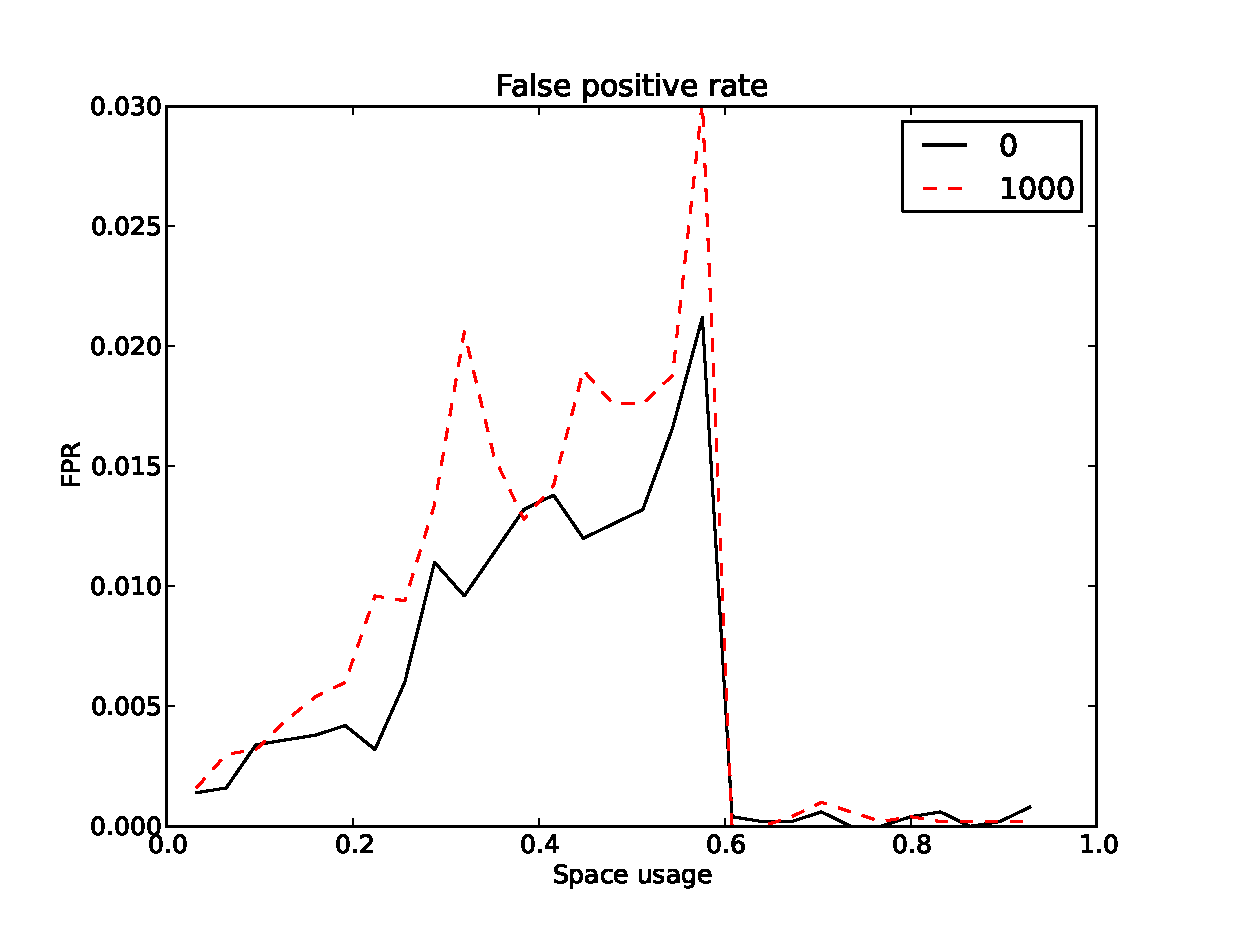
\includegraphics[width=.95\linewidth]{wildcard_1000_FPR1}
\end{subfigure}%
\begin{subfigure}{.5\textwidth}
  \centering
  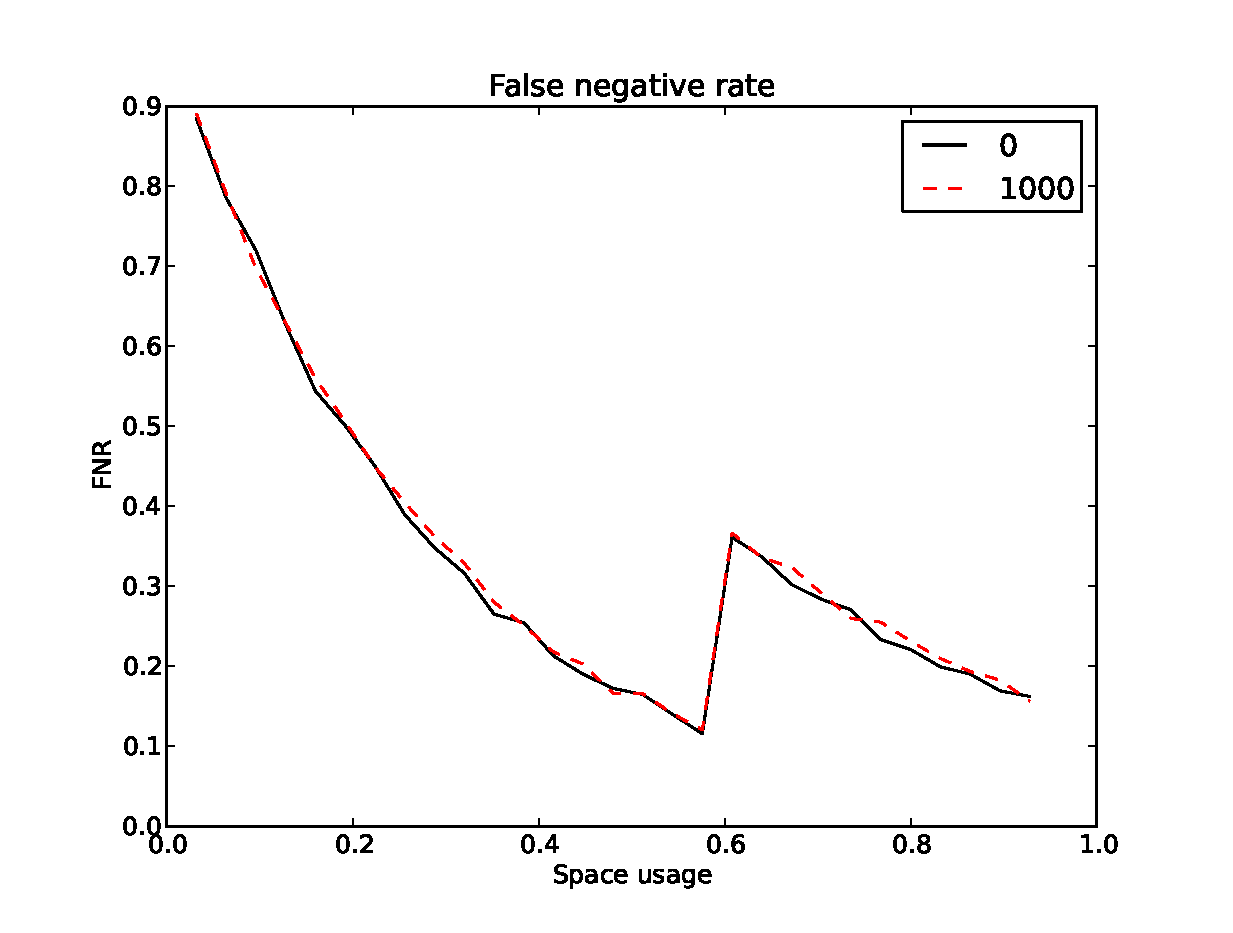
\includegraphics[width=.95\linewidth]{wildcard_1000_FNR1}
\end{subfigure}
\caption{The observed false positive and false negative rates for $n$ = 1000, $l$ = 65536, $\epsilon$ = 0.1, and $\delta$ = 0.4, with 2 different lengths of $W$}
\label{fig:w-fpnr}
\end{figure}

%performance
We have implemented wildcard search, and measured the actual performance of querying the DSBF with wildcards. The following experiments are carried out with the parameters\footnote{the remaining parameters are calculated as per \cite{paper:harvard}}: $l = 100, n = 100, k = 20, \epsilon=0.1, \delta=0.4$.

Figure \ref{fig:w-perf}a shows the performance of naïve approach 2 (red) against improved approach 2 (black), as the fraction of wildcarded bits increases. The graph shows that they both exhibit exponential growth, as expected, but that the improved version grows significantly slower, allowing for more wildcarded bits without significant loss of performance.

Figure \ref{fig:w-perf}b shows the performance gained by short-circuiting sub-queries. As expected, it exhibits the same asymptotical growth, but improves the performance slightly overall.

\begin{figure}[H]
\centering
\begin{subfigure}{.5\textwidth}
  \label{fig:w-query-performance}
  \centering
  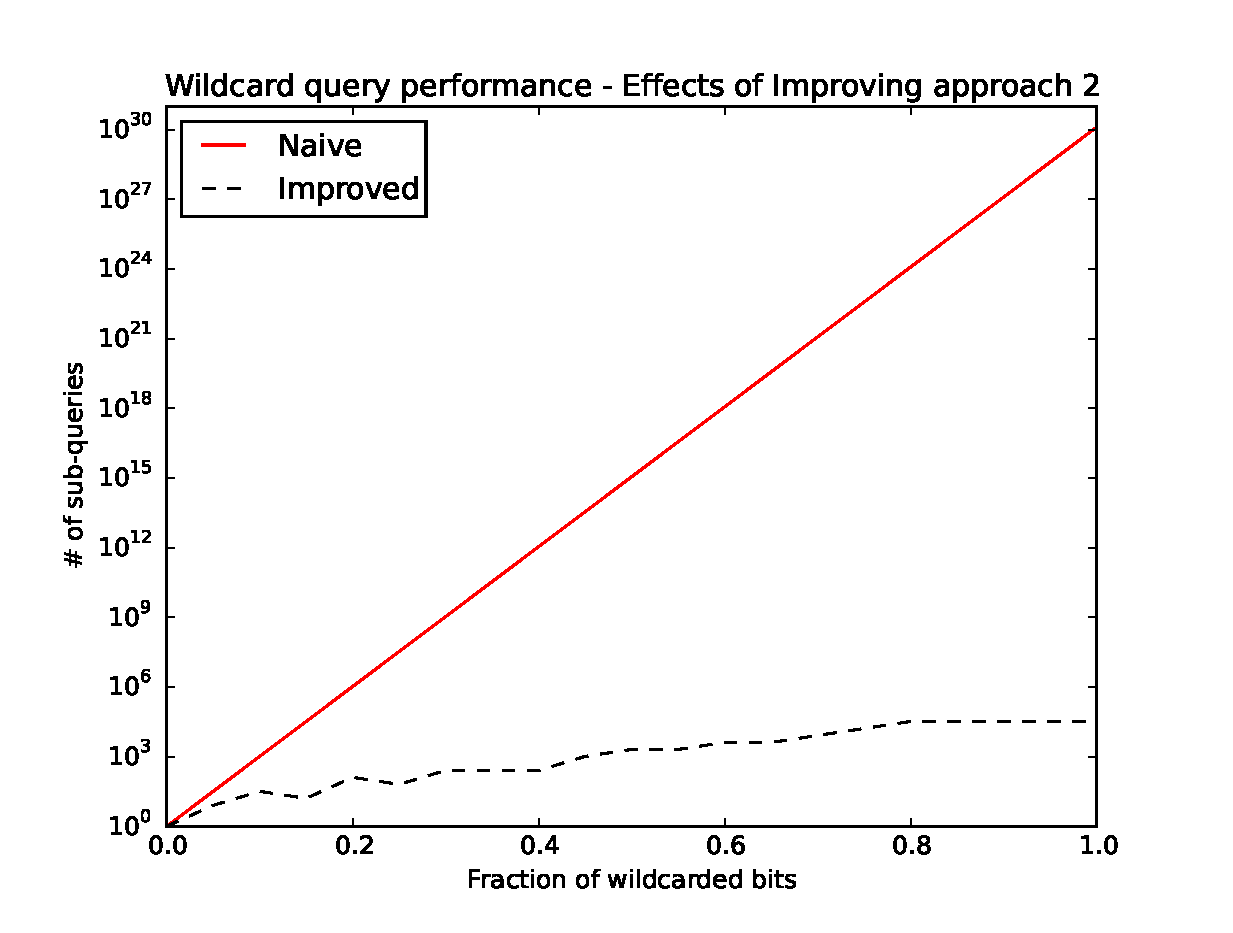
\includegraphics[width=.95\linewidth]{work_over_wildcards_approaches}
  \caption{}
\end{subfigure}%
\begin{subfigure}{.5\textwidth}
  \label{fig:w-short-circuit}
  \centering
  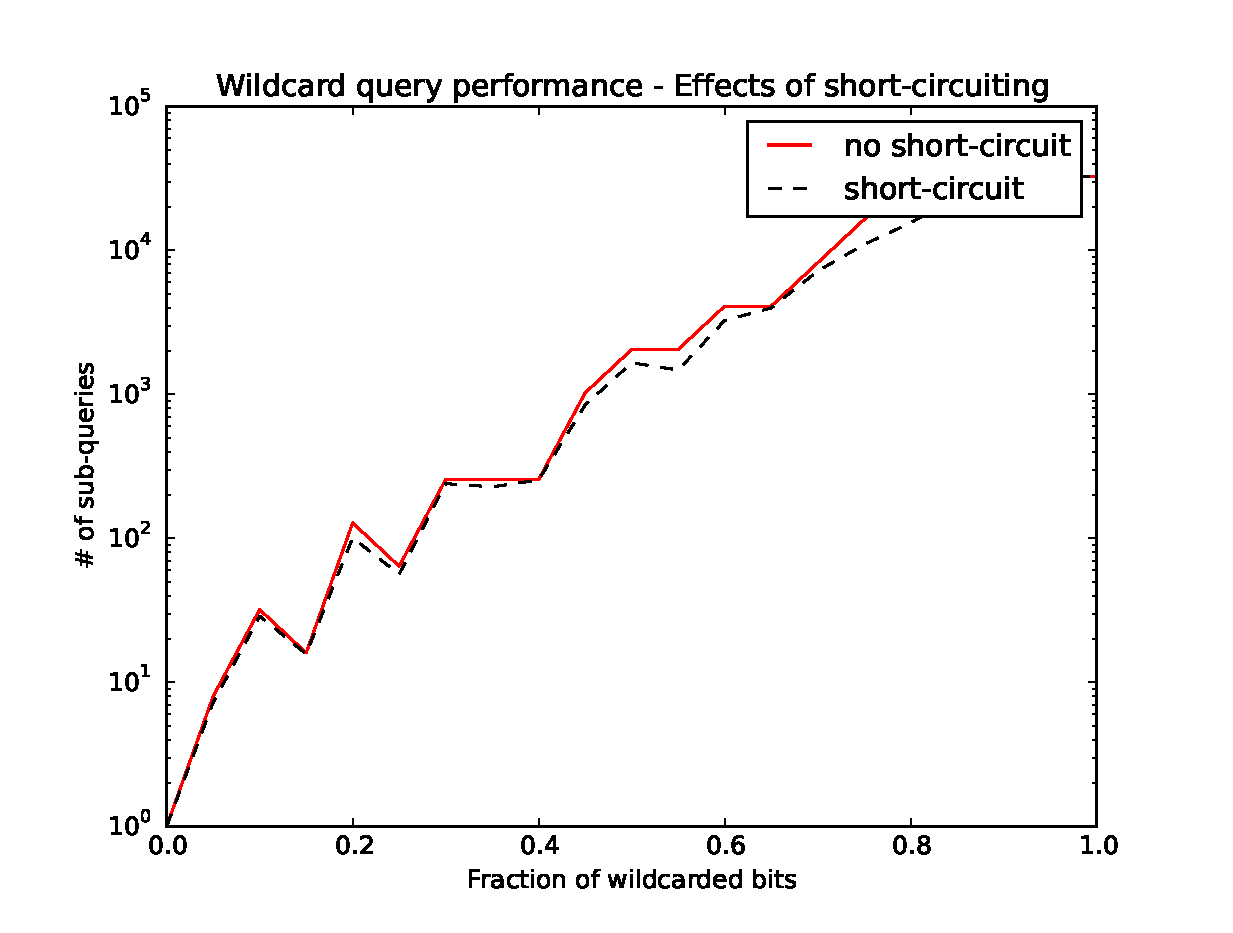
\includegraphics[width=.95\linewidth]{work_over_wildcards_short-circuit}
  \caption{}
\end{subfigure}
  \caption{Wildcard Search - Performance measurements}
  \label{fig:w-perf}
\end{figure}


\section{Conclusion}
% Vi har ændret på pladsen ved at gøre k større. Ville vi få værre/bedre resultater hvis vi varierede $m$?

%In this paper we have implemented the Distance Sensitive Bloom Filter\cite{paper:harvard} as presented by Kirsch \& Mitzenmacher. We have been able to roughly reproduce their results, regarding accuracy.
In this paper, we have introduced the Balanced LSH Bit Sampling method which aims to avoid skewed bit sampling. We have shown this to be a clear improvement for small problem instances, but expect the usefulness to decrease with growing problem sizes.\\

We have introduced a method to eliminate false negatives, at the cost of an increased probability of false positives. We have have argued that this is only useful for very small values of $\epsilon$, which makes it impractical for real-world applications.\\

Finally we have introduced an extension to the DSBF that allows for queries with wildcards. Wildcard queries expands the real-world applications of the Distance-Sensitive Bloom Filter, without increasing the space usage or true positive rate. This comes at the cost of a query time complexity, and false positive rate, that is exponential in the number of wildcards. We show that if the number of wildcards is sufficiently small, a wildcard query will run in expected constant time.\\

All source code is freely available at: \\\url{https://github.com/MartinFaartoft/similarity-filters}

\newpage

\begin{thebibliography}{}

\bibitem{paper:harvard}
Adam Kirsch, Michael Mitzenmacher
"Distance-Sensitive Bloom Filters", In Proceedings of the Eighth Workshop on Algorithm Engineering and Experiments (ALENEX), 2006

\bibitem{paper:hua}
Yu Hua, Bin Xiao, Bharadwaj Veeravalli, Dan Feng, "Locality-Sensitive Bloom Filter for Approximate Membership Query", IEEE Transactions on Computers, Vol. 61, No. 6, 2012


\bibitem{paper:bloom}
Flavio Bonomi, Michael Mitzenmacher, Rina Panigrahy, Sushil Singh, and George Varghese
"An Improved Construction for Counting Bloom Filters"

\end{thebibliography}

%code in appendix
\section*{Appendix}
\appendix
\section{Experiments}\label{appendix:experiments}
\begin{figure}[H]
\centering
\begin{subfigure}{.5\textwidth}
  \centering
  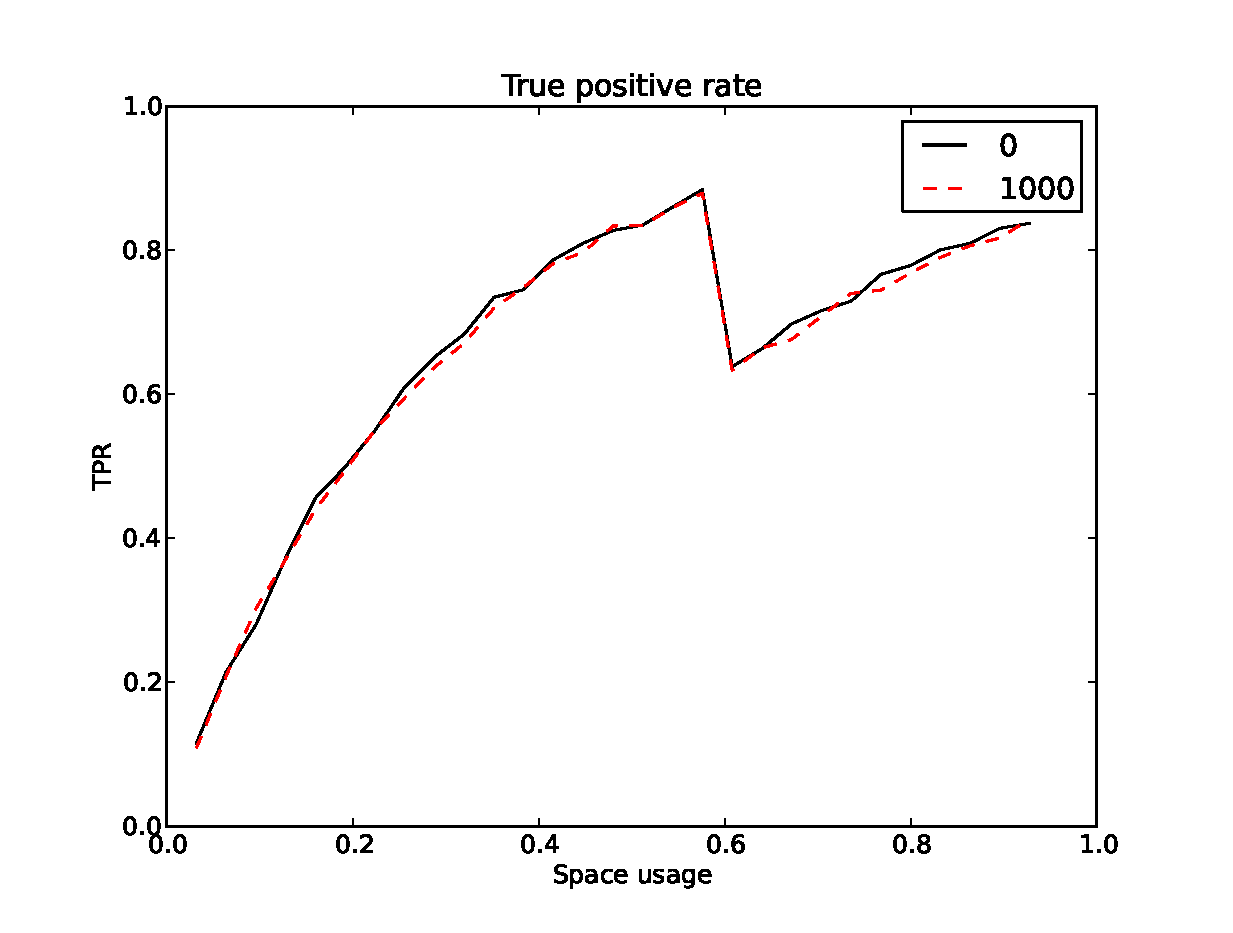
\includegraphics[width=.95\linewidth]{wildcard_1000_TPR1}
\end{subfigure}%
\begin{subfigure}{.5\textwidth}
  \centering
  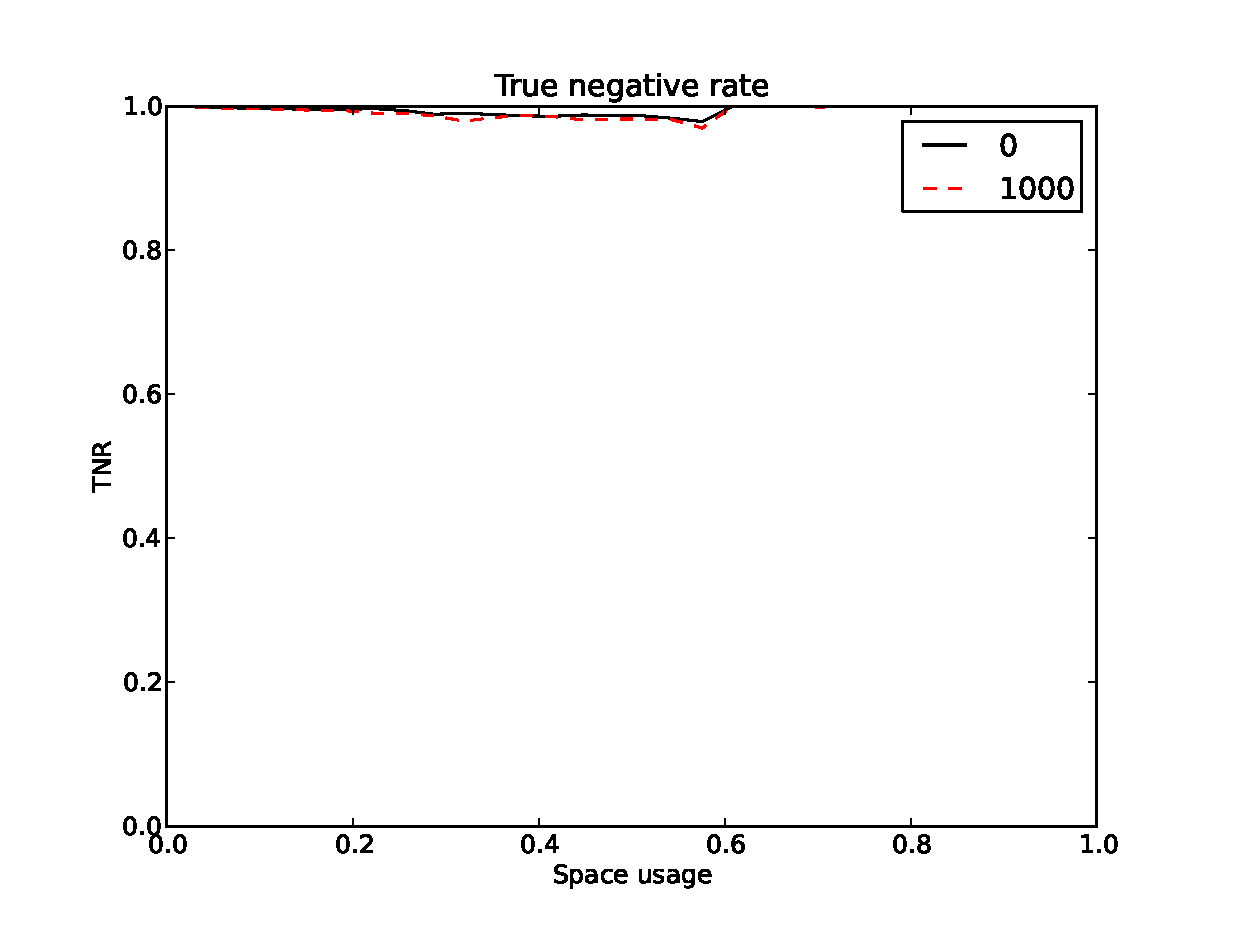
\includegraphics[width=.95\linewidth]{wildcard_1000_TNR1}
\end{subfigure}
\caption{The observed true positive and true negative rates for $n$ = 1000, $l$ = 65536, $\epsilon$ = 0.1, and $\delta$ = 0.4, with 2 different lengths of $W$}
\label{fig:w-tpnr}
\end{figure}

%\lstinputlisting[language=Python]{../src/dsbf.py}


\end{document}
